\chapter{Experiments}
\label{chap:experiments}
This chapter presents the results of eight sets of experiments for the implementation. The first experiment profiles the execution time of each phase on GPU. The second experiment focus on each optimization techniques. The third experiment compares the performance of CPU and GPU version. The fourth experiment shows the scalability of our implementation. The fifth and the sixth experiments compares the different testcases with different degree of coverage of rectangles and proportion of right triangles respectively. The seventh experiment investigates the results for different setting in checking memeory for windows (group). The eighth experiment discusses the sampling method to estimate the value of $\beta$.

The CPU used in the experiments is Intel Core i7-5820K, and the GPU is GeForce GTX 750 Ti with 4 GB global memory and its compute capability is 5.0. Each block has 48 KB shared memory and 65536 32 bits registers. We also use the GeForce GTX 1080 Ti with 11 GB global memory and its compute capabibity is 6.1. Each block has 96 KB shared memory and 65536 32 bits registers. We use two testcase in the experiment, their cell’s boundary is (0, 0) to (4700000, 4500000) and the number of total rectangles is both ten million. The lengths of rectangles are both one thousand in testcase 1. Contrary with it, the lengths of rectangles in testcase 2 are from one hundred to twenty thousand one hundred. the difference between two testcase is degree of coverage.

\section{Computing time of each phase}
From table \ref{table:5_1} to table \ref{table:5_8} show the profiles of the computing time on GPU for testcase 1 and testcase 2 respectively. The values in brackets which connected after the testcase are window size and window stride respectively. Multi-sweep-line (MSL) version is multi-slab version with all optimizations we described before. To focus on our implementations, all our three versions use fast segmented sort.

\begin{table}[!h]
\centering
\newcommand{\tabincell}[2]{\begin{tabular}{@{}#1@{}}#2\end{tabular}}
\begin{tabular}{| l | c | c | c | c | c | c | c | c |} 
 \hline
  & sampling & counting & mapping & sorting & \tabincell{c}{counting\\range} & \tabincell{c}{mapping\\range} & computing & total\\ [0.5ex] \hline
  baseline &  & 108 & 105 & 41 &  &  & 3,639 & 3,893\\ \hline
  multi-slab & 777 & 112 & 114 & 101 & 310 & 275 & 836 & 2,525\\ \hline
  MSL & 778 & 112 & 114 & 101 & 230 & 410 & 199 & 1,944\\ \hline
\end{tabular}
\caption{The computing time of each phase for testcase1(10000, 10000) on GTX 750 Ti(unit: ms)}
\label{table:5_1}
\end{table}

\begin{table}[!h]
\centering
\newcommand{\tabincell}[2]{\begin{tabular}{@{}#1@{}}#2\end{tabular}}
\begin{tabular}{| l | c | c | c | c | c | c | c | c |} 
 \hline
  & sampling & counting & mapping & sorting & \tabincell{c}{counting\\range} & \tabincell{c}{mapping\\range} & computing & total\\ [0.5ex] \hline
  baseline &  & 208 & 215 & 151 &  &  & 14,423 & 14,997\\ \hline
  multi-slab & 777 & 225 & 231 & 389 & 1,281 & 1,020 & 3,302 & 7,225\\ \hline
  MSL & 778 & 223 & 231 & 390 & 861 & 1,636 & 805 & 4,924\\ \hline
\end{tabular}
\caption{The computing time of each phase for testcase1(10000, 5000) on GTX 750 Ti(unit: ms)}
\label{table:5_2}
\end{table}

\begin{table}[!h]
\centering
\newcommand{\tabincell}[2]{\begin{tabular}{@{}#1@{}}#2\end{tabular}}
\begin{tabular}{| l | c | c | c | c | c | c | c | c |} 
 \hline
  & sampling & counting & mapping & sorting & \tabincell{c}{counting\\range} & \tabincell{c}{mapping\\range} & computing & total\\ [0.5ex] \hline
  baseline &  & 139 & 144 & 158 &  &  & 21,631 & 22,072\\ \hline
  multi-slab & 777 & 143 & 156 & 299 & 1,813 & 1,599 & 2,272 & 7,059\\ \hline
  MSL & 775 & 142 & 158 & 300 & 567 & 1,187 & 1,391 & 4,520\\ \hline
\end{tabular}
\caption{The computing time of each phase for testcase2(10000, 10000) on GTX 750 Ti (unit: ms)}
\label{table:5_3}
\end{table}

\begin{table}[!h]
\centering
\newcommand{\tabincell}[2]{\begin{tabular}{@{}#1@{}}#2\end{tabular}}
\begin{tabular}{| l | c | c | c | c | c | c | c | c |} 
 \hline
  & sampling & counting & mapping & sorting & \tabincell{c}{counting\\range} & \tabincell{c}{mapping\\range} & computing & total\\ [0.5ex] \hline
  baseline &  & 281 & 371 & 619 &  &  & 89,469 & 90,740\\ \hline
  multi-slab & 777 & 292 & 391 & 1,183 & 7,255 & 6,593 & 8,856 & 25,347\\ \hline
  MSL & 776 & 293 & 391 & 1,184 & 2,303 & 4,751 & 5,542 & 15,240\\ \hline
\end{tabular}
\caption{The computing time of each phase for testcase2(10000, 5000) on GTX 750 Ti (unit: ms)}
\label{table:5_4}
\end{table}

\begin{table}[!h]
\centering
\newcommand{\tabincell}[2]{\begin{tabular}{@{}#1@{}}#2\end{tabular}}
\begin{tabular}{| l | c | c | c | c | c | c | c | c |} 
 \hline
  & sampling & counting & mapping & sorting & \tabincell{c}{counting\\range} & \tabincell{c}{mapping\\range} & computing & total\\ [0.5ex] \hline
  baseline &  & 11 & 12 & 17 &  &  & 583 & 623\\ \hline
  multi-slab & 82 & 10 & 10 & 31 & 44 & 46 & 102 & 325\\ \hline
  MSL & 81 & 9 & 10 & 27 & 34 & 36 & 25 & 222\\ \hline
\end{tabular}
\caption{The computing time of each phase for testcase1(10000, 10000) on GTX 1080 Ti(unit: ms)}
\label{table:5_5}
\end{table}

\begin{table}[!h]
\centering
\newcommand{\tabincell}[2]{\begin{tabular}{@{}#1@{}}#2\end{tabular}}
\begin{tabular}{| l | c | c | c | c | c | c | c | c |} 
 \hline
  & sampling & counting & mapping & sorting & \tabincell{c}{counting\\range} & \tabincell{c}{mapping\\range} & computing & total\\ [0.5ex] \hline
  baseline &  & 21 & 24 & 63 &  &  & 2,068 & 2,176\\ \hline
  multi-slab & 83 & 20 & 23 & 113 & 167 & 169 & 400 & 975\\ \hline
  MSL & 81 & 18 & 21 & 114 & 114 & 145 & 95 & 588\\ \hline
\end{tabular}
\caption{The computing time of each phase for testcase1(10000, 5000) on GTX 1080 Ti(unit: ms)}
\label{table:5_6}
\end{table}

\begin{table}[!h]
\centering
\newcommand{\tabincell}[2]{\begin{tabular}{@{}#1@{}}#2\end{tabular}}
\begin{tabular}{| l | c | c | c | c | c | c | c | c |} 
 \hline
  & sampling & counting & mapping & sorting & \tabincell{c}{counting\\range} & \tabincell{c}{mapping\\range} & computing & total\\ [0.5ex] \hline
  baseline &  & 14 & 18 & 56 &  &  & 3,274 & 3,362\\ \hline
  multi-slab & 85 & 13 & 16 & 74 & 158 & 1,678 & 767 & 2,791\\ \hline
  MSL & 81 & 13 & 16 & 81 & 77 & 99 & 238 & 605\\ \hline
\end{tabular}
\caption{The computing time of each phase for testcase2(10000, 10000) on GTX 1080 Ti (unit: ms)}
\label{table:5_7}
\end{table}

\begin{table}[!h]
\centering
\newcommand{\tabincell}[2]{\begin{tabular}{@{}#1@{}}#2\end{tabular}}
\begin{tabular}{| l | c | c | c | c | c | c | c | c |} 
 \hline
  & sampling & counting & mapping & sorting & \tabincell{c}{counting\\range} & \tabincell{c}{mapping\\range} & computing & total\\ [0.5ex] \hline
  baseline &  & 30 & 48 & 193 &  &  & 12,848 & 13,119\\ \hline
  multi-slab & 83 & 27 & 47 & 294 & 616 & 6,645 & 2,928 & 10,640\\ \hline
  MSL & 75 & 23 & 41 & 291 & 281 & 395 & 999 & 2,105\\ \hline
\end{tabular}
\caption{The computing time of each phase for testcase2(10000, 5000) on GTX 1080 Ti (unit: ms)}
\label{table:5_8}
\end{table}

Comparing tables \ref{table:5_1} and \ref{table:5_3}, which are using different testcase, one can find that computing time after sorting step is increased. The reason for this condition is because of the degree of overlap is more serious in testcase 2. The computing time before sorting step almost nothing changes because the total number of rectangles is same between two testcases.

\section{Optimization techniques}

\subsection{Fast segmented sort}
Table \ref{table:5_9} and table \ref{table:5_10} show the sorting performance of using fast segmented sort. It is almost 9 $\sim$ 90 times faster than origin sorting, which we using thrust in kernel function.
\begin{table}[h!]
\centering
\begin{tabular}{| l | c | c |} 
 \hline
  & Thrust sort & Fast segmented sort \\ [0.5ex] \hline
  Testcase 1 (10000, 10000) & 922 & 101\\ \hline
  Testcase 1 (10000, 5000) & 3,456 & 390\\ \hline
  Testcase 2 (10000, 10000) & 2,880 & 300\\ \hline
  Testcase 2 (10000, 5000) & 8,013 & 1,184\\ \hline
\end{tabular}
\caption{The computing time of sorting on GTX 750 Ti (unit: ms)}
\label{table:5_9}
\end{table}

\begin{table}[h!]
\centering
\begin{tabular}{| l | c | c |} 
 \hline
  & Thrust sort & Fast segmented sort \\ [0.5ex] \hline
  Testcase 1 (10000, 10000) & 2,567 & 27\\ \hline
  Testcase 1 (10000, 5000) & 6,625 & 114\\ \hline
  Testcase 2 (10000, 10000) & 7,365 & 81\\ \hline
  Testcase 2 (10000, 5000) & 12,319 & 291\\ \hline
\end{tabular}
\caption{The computing time of sorting on GTX 1080 Ti (unit: ms)}
\label{table:5_10}
\end{table}

\subsection{Reducing atomic instruction}
Table \ref{table:5_11} and table \ref{table:5_12} show the difference of reducing atomic instruction in counting range phase. It can speedup 1.2 $\sim$ 3 times in testcase 1 and testcase 2.
\begin{table}[!h]
\centering
\begin{tabular}{| l | c | c |} 
 \hline
  & With atomic instruction & Without atomic instruction \\ [0.5ex] \hline
  Testcase 1 (10000, 10000) & 311 & 230\\ \hline
  Testcase 1 (10000, 5000) & 1,211 & 861\\ \hline
  Testcase 2 (10000, 10000) & 1,817 & 567\\ \hline
  Testcase 2 (10000, 5000) & 7,358 & 2,303\\ \hline
\end{tabular}
\caption{The computing time of counting range phase on GTX 750 Ti (unit: ms)}
\label{table:5_11}
\end{table}

\begin{table}[!h]
\centering
\begin{tabular}{| l | c | c |} 
 \hline
  & With atomic instruction & Without atomic instruction \\ [0.5ex] \hline
  Testcase 1 (10000, 10000) & 43 & 34\\ \hline
  Testcase 1 (10000, 5000) & 166 & 114\\ \hline
  Testcase 2 (10000, 10000) & 157 & 77\\ \hline
  Testcase 2 (10000, 5000) & 627 & 281\\ \hline
\end{tabular}
\caption{The computing time of counting range phase on GTX 1080 Ti (unit: ms)}
\label{table:5_12}
\end{table}

\subsection{Multi-sweep-line algorithm with load balance}
Table \ref{table:5_13} and table \ref{table:5_14} show the performance of using multi-sweep-line algorithm and load balance we presented in this thesis. It can improve computing phase approximate 1.6 $\sin$ 4 times in testcase 1 and testcase 2.
\begin{table}[!h]
\centering
\begin{tabular}{| l | c | c | c |} 
 \hline
  & Origin  & Multi-sweep-line without load balance & Multi-sweep-line \\ [0.5ex] \hline
  Testcase 1 (10000, 10000) & 835 & 255 & 199\\ \hline
  Testcase 1 (10000, 5000) & 3,279 & 1,017 & 804\\ \hline
  Testcase 2 (10000, 10000) & 2,270 & 1,749 & 1,391\\ \hline
  Testcase 2 (10000, 5000) & 8,917 & 6,980 & 5,542\\ \hline
\end{tabular}
\caption{The computing time of computing phase on GTX 750 Ti (unit: ms)}
\label{table:5_13}
\end{table}

\begin{table}[!h]
\centering
\begin{tabular}{| l | c | c | c |} 
 \hline
  & Origin  & Multi-sweep-line without load balance & Multi-sweep-line \\ [0.5ex] \hline
  Testcase 1 (10000, 10000) & 102 & 31 & 25\\ \hline
  Testcase 1 (10000, 5000) & 407 & 122 & 95\\ \hline
  Testcase 2 (10000, 10000) & 770 & 314 & 238\\ \hline
  Testcase 2 (10000, 5000) & 2,927 & 1,283 & 999\\ \hline
\end{tabular}
\caption{The computing time of computing phase on GTX 1080 Ti (unit: ms)}
\label{table:5_14}
\end{table}

\section{Comparison between GPU and CPU}
Fig. \ref{fig:fig_5_1}, Fig. \ref{fig:fig_5_2}, Fig. \ref{fig:fig_5_3}, and Fig. \ref{fig:fig_5_4} show the computing time of CPU and GPU version. The sequence CPU versions we used are provided by AnaGlobe Technology, Inc. They have two implementations. The first one is to compute general polygon union area, like boost geometry, it overlay all polygons and generate several new polygons, and then compute their area. The second one is optimized to calculate density (union), it decompose all non-rectilinear polygons into vertical trapezoids, and merge overlapped vertical trapezoids into non-overlapped vertical trapezoids, finally it can be easily to calculate vertical trapezoids area. We also tried to transform our GPU version algorithm to sequence code, but it is slower than the code provided by AnaGlobe Technology, Inc. For this reason, we only compare our implementation with their sequence codes. We do not show profile information because we cannot profile detail of their implementations. From Fig. \ref{fig:fig_5_1} to Fig. \ref{fig:fig_5_4} show that the total computing time of GPU versions is faster than CPU version and (10000, 10000) means the length of windows and the stride of each windows are both ten thousand. MSL speedup more than 20 and  77 times than sequence code on GTX 750 Ti and GTX 1080 Ti. It should be noted that the sampling time is same in multi-slab version and MSL version with different window setting, so the speedup in (10000, 10000) setting is not more obvious than (10000, 5000) due to the total computing time is smaller.

\begin{figure}[h]
    \centering
    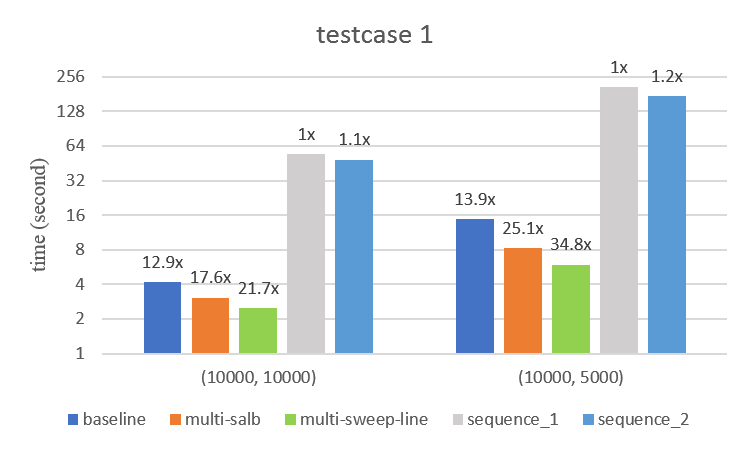
\includegraphics[scale=0.7]{image/fig_5_1}
    \caption{The computing time of CPU and GPU version in testcase 1 on GTX 750 Ti}
    \label{fig:fig_5_1}
\end{figure}

\begin{figure}[h]
    \centering
    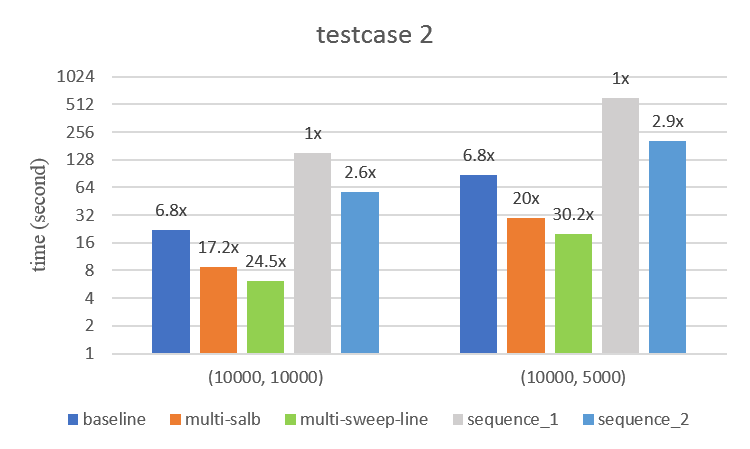
\includegraphics[scale=0.7]{image/fig_5_2}
    \caption{The computing time of CPU and GPU version in testcase 2 on GTX 750 Ti}
    \label{fig:fig_5_2}
\end{figure}

\begin{figure}[h]
    \centering
    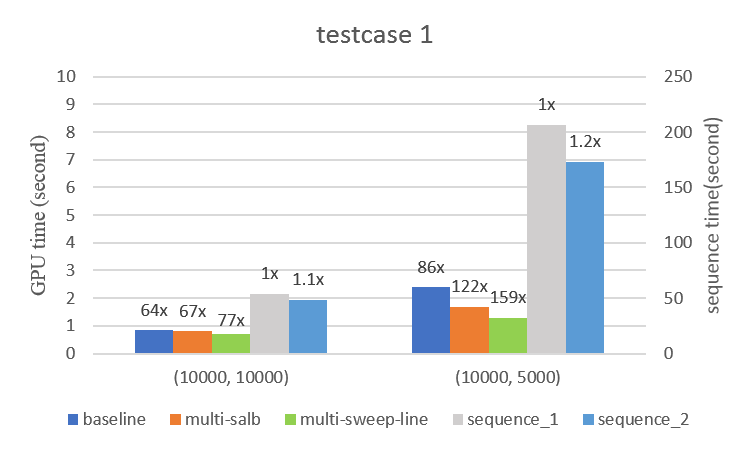
\includegraphics[scale=0.7]{image/fig_5_3}
    \caption{The computing time of CPU and GPU version in testcase 1 on GTX 1080 Ti}
    \label{fig:fig_5_3}
\end{figure}

\begin{figure}[h]
    \centering
    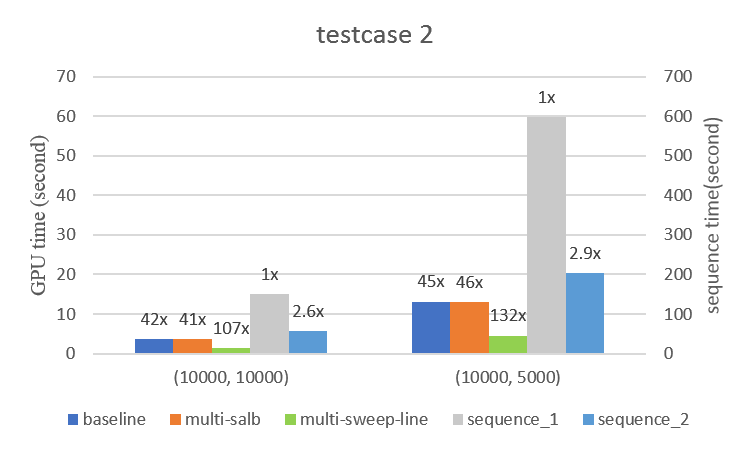
\includegraphics[scale=0.7]{image/fig_5_4}
    \caption{The computing time of CPU and GPU version in testcase 2 on GTX 1080 Ti}
    \label{fig:fig_5_4}
\end{figure}

\section{Multiple GPUs (scalability)}
Fig. \ref{fig:fig_5_5} and Fig. \ref{fig:fig_5_6} show the scalability of using multiple GPUs. We use K80 from one to four on one device node in the cluster. We only calculate the execution time except the time of rectangle information copy from host to device because the communication time between host node and device node is slower than computing time in GPUs.

\begin{figure}[h]
    \centering
    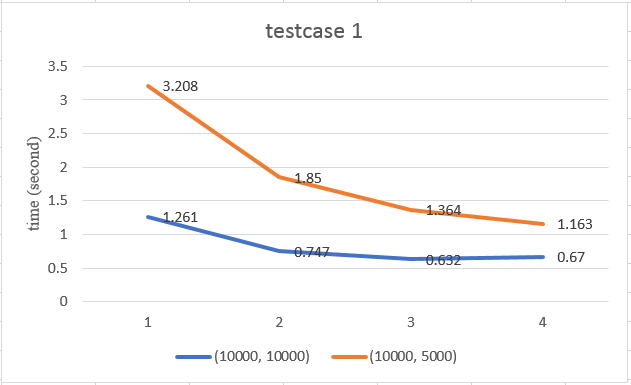
\includegraphics[scale=0.7]{image/fig_5_5}
    \caption{The strong scalability of Multi-sweep-line in testcase 1}
    \label{fig:fig_5_5}
\end{figure}

\begin{figure}[h]
    \centering
    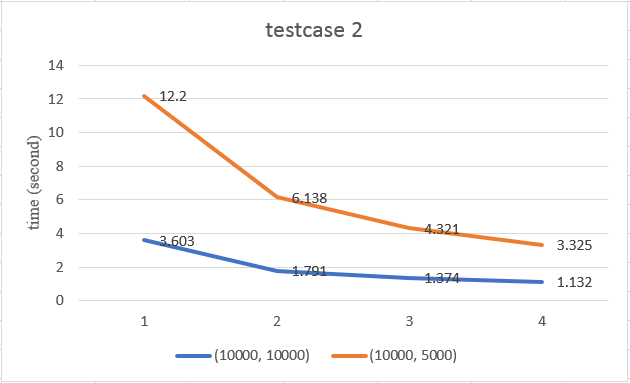
\includegraphics[scale=0.7]{image/fig_5_6}
    \caption{The strong scalability of Multi-sweep-line in testcase 2}
    \label{fig:fig_5_6}
\end{figure}

Our process uses less time when we using more GPUs, it provides strong scalability. The execution time between using 3 and 4 GPUs is similar when window size equals to window stride (blue line) in testcase 1 because the degree of coverage is not uniform and we equally partition the cell.

\section{Comparison between testcases with different degree of coverage}
From Fig. \ref{fig:fig_5_7} to Fig. \ref{fig:fig_5_10} show the comparison between testcases with different degree of coverage. When win\_stride is equal to 10000, the speedup is only 20 times and 70 times in GTX 750 Ti and GTX 1080 Ti. And the speedup is 30 times and 120 times in GTX 750 Ti and GTX 1080 Ti when win\_stride is equal to 5000. The reason for this condition is that the computing time of allocate and sampling are constant.

\begin{figure}[!h]
    \centering
    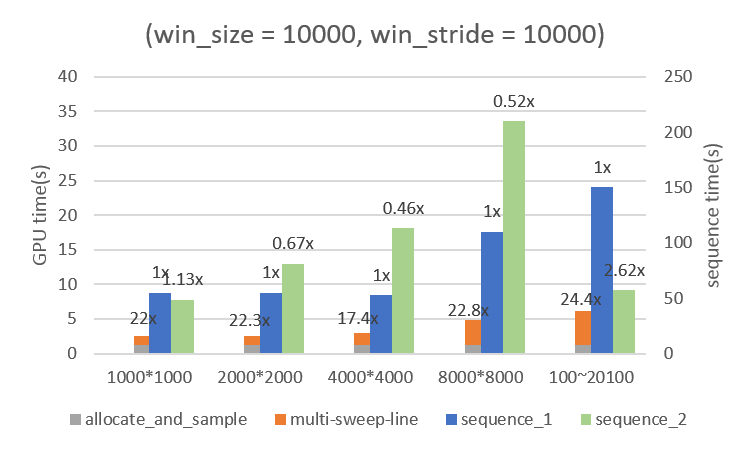
\includegraphics[scale=0.7]{image/fig_5_7}
    \caption{The computing time of multi-sweep-line and sequences in testcases with different degree of coverage (win\_size = 10000, win\_stride = 10000) on GTX 750 Ti}
    \label{fig:fig_5_7}
\end{figure}

\begin{figure}[!h]
    \centering
    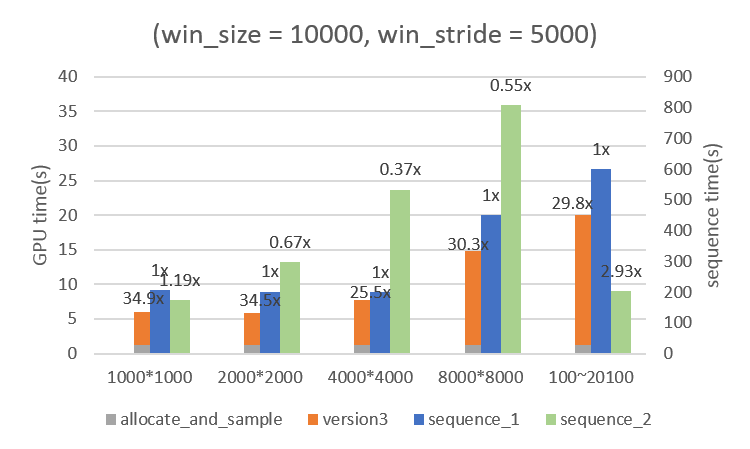
\includegraphics[scale=0.7]{image/fig_5_8}
    \caption{The computing time of multi-sweep-line and sequences in testcases with different degree of coverage (win\_size = 10000, win\_stride = 5000) on GTX 750 Ti}
    \label{fig:fig_5_8}
\end{figure}

\begin{figure}[!h]
    \centering
    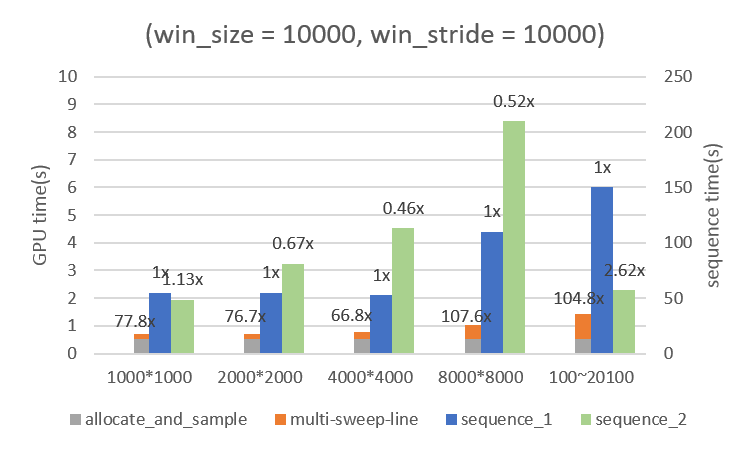
\includegraphics[scale=0.7]{image/fig_5_9}
    \caption{The computing time of multi-sweep-line and sequences in testcases with different degree of coverage (win\_size = 10000, win\_stride = 10000) on GTX 1080 Ti}
    \label{fig:fig_5_9}
\end{figure}

\begin{figure}[!h]
    \centering
    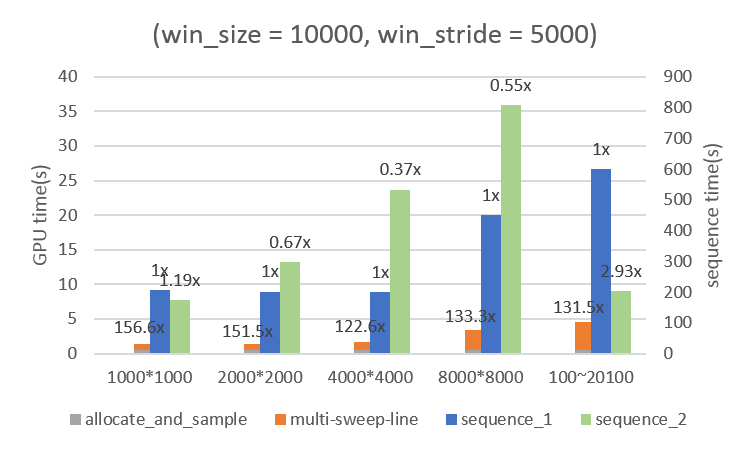
\includegraphics[scale=0.7]{image/fig_5_10}
    \caption{The computing time of multi-sweep-line and sequences in testcases with different degree of coverage (win\_size = 10000, win\_stride = 5000) on GTX 1080 Ti}
    \label{fig:fig_5_10}
\end{figure}

\section{Comparison between testcases with different proportion of right triangles}
From Fig. \ref{fig:fig_5_11} to Fig. \ref{fig:fig_5_14} show the comparison between testcases with different proportion of triangles. If we use OpenMP to accelerate the calculating time of triangles on CPU, it can be almost completely overlapping in the computing time on GPU.

\begin{figure}[!h]
    \centering
    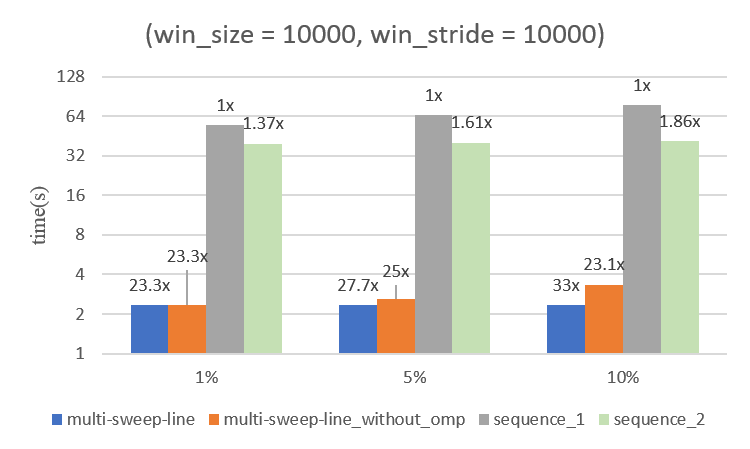
\includegraphics[scale=0.7]{image/fig_5_11}
    \caption{The computing time of multi-sweep-line, multi-sweep-line without OpenMP and sequences in testcases with different proportion of triangles (win\_size = 10000, win\_stride = 10000) on GTX 750 Ti}
    \label{fig:fig_5_11}
\end{figure}

\begin{figure}[!h]
    \centering
    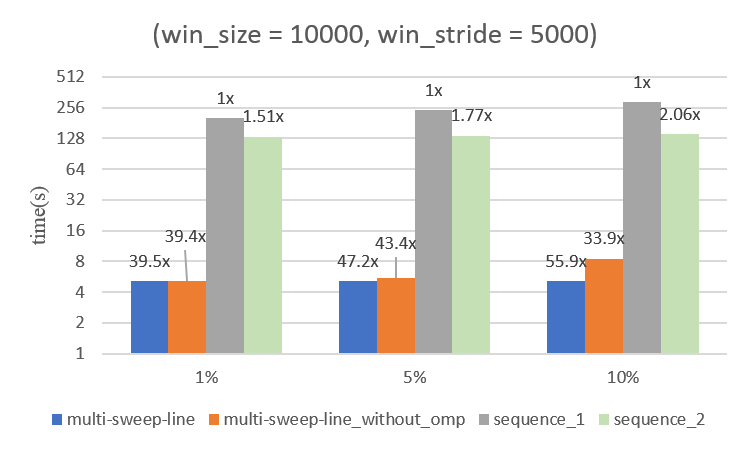
\includegraphics[scale=0.7]{image/fig_5_12}
    \caption{The computing time of multi-sweep-line, multi-sweep-line without OpenMP and sequences in testcases with different proportion of triangles (win\_size = 10000, win\_stride = 5000) on GTX 750 Ti}
    \label{fig:fig_5_12}
\end{figure}

\begin{figure}[!h]
    \centering
    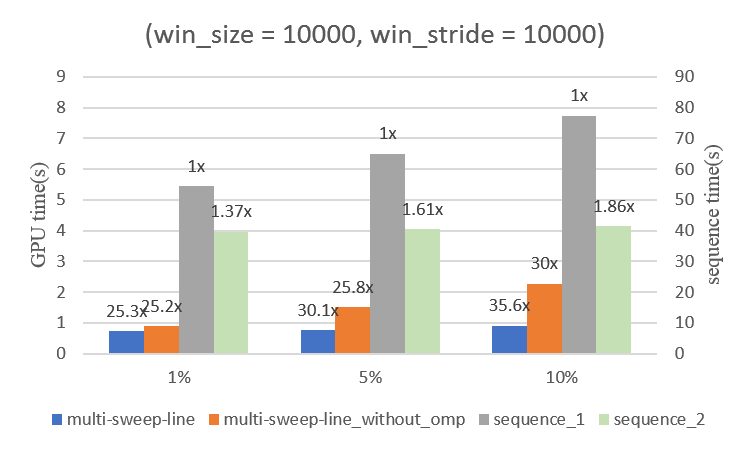
\includegraphics[scale=0.7]{image/fig_5_13}
    \caption{The computing time of multi-sweep-line, multi-sweep-line without OpenMP and sequences in testcases with different proportion of triangles (win\_size = 10000, win\_stride = 10000) on GTX 1080 Ti}
    \label{fig:fig_5_13}
\end{figure}

\begin{figure}[!h]
    \centering
    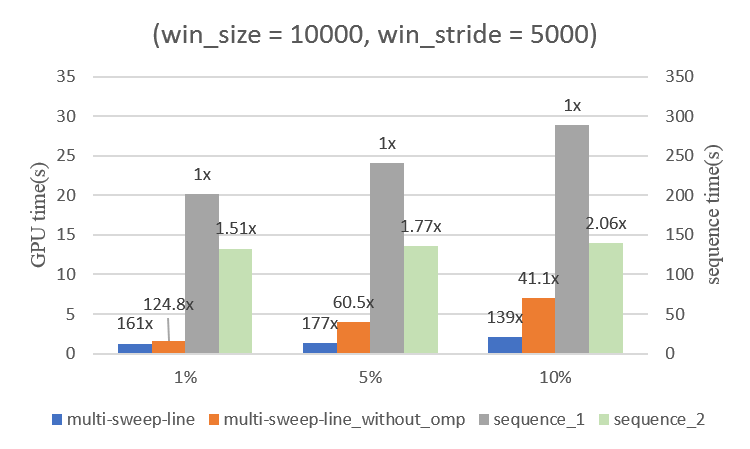
\includegraphics[scale=0.7]{image/fig_5_14}
    \caption{The computing time of multi-sweep-line, multi-sweep-line without OpenMP and sequences in testcases with different proportion of triangles (win\_size = 10000, win\_stride = 5000) on GTX 1080 Ti}
    \label{fig:fig_5_14}
\end{figure}

\section{Discussion for the checking memory for windows (group)}
Table \ref{table:5_15} shows the results for different setting in checking memory for windows. The total in table means the process checks total memory usage including additional array (\textit{range counter array}, \textit{range offset array}, and \textit{range rectangle array}) and partition task. The value 1/600 means the process does not consider whole these three arrays, it only checks other memory usage and these three arrays divided by 600. We can see that there is no significant differences on 1080 Ti, but it is slower on 750 Ti if the process checks whole memory usage. The reason for this situation is that three additional array is larger than global memory and it will make process partition the task into many subtask. The computing time of counting phase and mapping phase is increasing. So we choose 1/400 in our process according to the experiment.

\begin{table}[!h]
\centering
\begin{tabular}{|c|l|c|l|c|}
\hline
\multicolumn{1}{|l|}{}   & \multicolumn{2}{l|}{testcase 1 (10000, 5000)} & \multicolumn{2}{l|}{testcase 2 (10000, 5000)} \\ \hline
\multirow{6}{*}{750 Ti}  & total & 7.202732 & total & 33.134935 \\ \cline{2-5} 
                         & 1/600 & 5.92086 & 1/600 & 20.283393 \\ \cline{2-5} 
                         & 1/500 & 5.929029 & 1/500 & 20.047735 \\ \cline{2-5} 
                         & 1/400 & 5.928557 & 1/400 & 20.040704 \\ \cline{2-5} 
                         & 1/300 & 5.92923 & 1/300 & 21.20294 \\ \cline{2-5} 
                         & 1/200 & 5.928677 & 1/200 & 21.364763 \\ \hline
\multirow{6}{*}{1080 Ti} & total & 1.416512 & total & 4.274711 \\ \cline{2-5} 
                         & 1/600 & 1.319576 & 1/600 & 4.527126 \\ \cline{2-5} 
                         & 1/500 & 1.315042 & 1/500 & 4.51068 \\ \cline{2-5} 
                         & 1/400 & 1.303876 & 1/400 & 4.567402 \\ \cline{2-5} 
                         & 1/300 & 1.307797 & 1/300 & 4.53494 \\ \cline{2-5} 
                         & 1/200 & 1.325864 & 1/200 & 4.505561 \\ \hline
\end{tabular}
\caption{The comparison results of checking memory for windows with different setting (unit: second)}
\label{table:5_15}
\end{table}

\section{Discussion for the sampling methods}
Table \ref{table:5_16} shows the results for different sampling method to estimate the number of rectangles in range rectangle array. Method 1 is using $\alpha$ to estimate the value of $\beta$ which we present in section 3.3.4; Method 2 is sampling to obtain not only $\alpha$ but also $\beta$. The difference means difference between the value we estimate and the real value in each testcase. Method 1 uses less time and small difference in testcase 2. The discrepancy between method 1 and method 2 in testcase 1 is similar (not consider positive or negative). We prefer to estimate larger number if difference is same, because we do not want to partition the task in next checking memory phase. Fig. \ref{fig:fig_5_15} shows the computing time of testcase 2 (win\_size = 10000, win\_stride = 5000) on GPU 750 Ti.

It should be noted that the process does not use $\beta$ in testcase 1 on GPU 750 Ti because the memory usage of testcase 1 is smaller than testcase 2.

\begin{table}[h!]
\centering
\begin{tabular}{| l | c | c | c |} 
 \hline
  & Method 1 (difference) & Method 2 (difference) & Real \\ [0.5ex] \hline
  Testcase 1 (10000, 10000) & 352,937,165 (65\%) & 81,626,040 (-61.68\%) & 213,021,830\\ \hline
  Testcase 1 (10000, 5000) & 1,414,292,101 (66.4\%) & 287,502,262 (-66.17\%) & 849,893,958\\ \hline
  Testcase 2 (10000, 10000) & 3,759,366,934 (-0.43\%) & 3,443,852,187 (-8.79\%) & 3,775,973,474\\ \hline
  Testcase 2 (10000, 5000) & 15,035,545,349 (-0.42\%) & 13,798,415,684 (-8.61\%) & 15,099,020,249\\ \hline
\end{tabular}
\caption{The comparison results of sampling methods (unit: rectangle)}
\label{table:5_16}
\end{table}

\begin{figure}[!h]
    \centering
    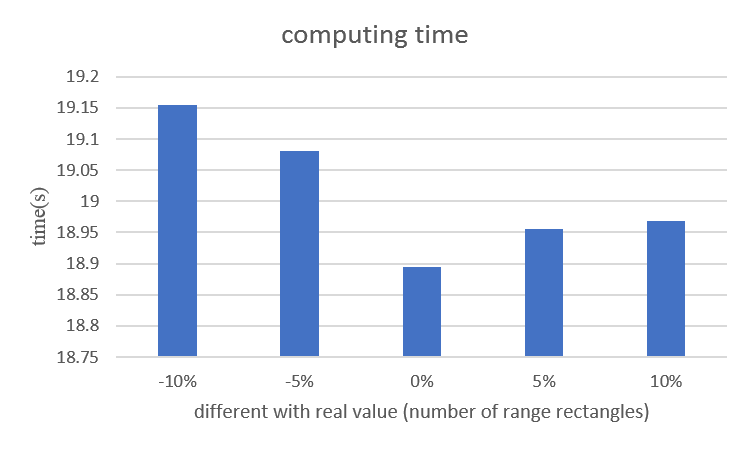
\includegraphics[scale=0.7]{image/fig_5_15}
    \caption{The computing time of different percentage with real value of range rectangle array (unit: rectangles)}
    \label{fig:fig_5_15}
\end{figure}